% Copyright 2004 by Till Tantau <tantau@users.sourceforge.net>.
%
% In principle, this file can be redistributed and/or modified under
% the terms of the GNU Public License, version 2.
%
% However, this file is supposed to be a template to be modified
% for your own needs. For this reason, if you use this file as a
% template and not specifically distribute it as part of a another
% package/program, I grant the extra permission to freely copy and
% modify this file as you see fit and even to delete this copyright
% notice. 

\documentclass{beamer}
% Replace the \documentclass declaration above
% with the following two lines to typeset your 
% lecture notes as a handout:
%\documentclass{article}
%\usepackage{beamerarticle}
\usepackage{hyperref}
\usepackage{fancybox}
% There are many different themes available for Beamer. A comprehensive
% list with examples is given here:
% http://deic.uab.es/~iblanes/beamer_gallery/index_by_theme.html
% You can uncomment the themes below if you would like to use a different
% one:
%\usetheme{AnnArbor}
%\usetheme{Antibes}
%\usetheme{Bergen}
%\usetheme{Berkeley}
%\usetheme{Berlin}
%\usetheme{Boadilla}
%\usetheme{boxes}
%\usetheme{CambridgeUS}
%\usetheme{Copenhagen}
%\usetheme{Darmstadt}
%\usetheme{default}
%\usetheme{Frankfurt}
\usetheme{Goettingen}
%\usetheme{Hannover}
%\usetheme{Ilmenau}
%\usetheme{JuanLesPins}
%\usetheme{Luebeck}
%\usetheme{Madrid}
%\usetheme{Malmoe}
%\usetheme{Marburg}
%\usetheme{Montpellier}
%\usetheme{PaloAlto}
%\usetheme{Pittsburgh}
%\usetheme{Rochester}
%\usetheme{Singapore}
%\usetheme{Szeged}
%\usetheme{Warsaw}

\title[C]{Programming with C}

% A subtitle is optional and this may be deleted
\subtitle{3. Introduction to Scientific Computing with Linux\\Part III. Basic Computing}

\author[Nidish, B. N.]{Nidish Narayanaa B\inst{1}}% \and S.~Another\inst{2}}
% - Give the names in the same order as the appear in the paper.
% - Use the \inst{?} command only if the authors have different
%   affiliation.

\institute[IIST] % (optional, but mostly needed)
{
  \inst{1}%
  Department of Aerospace Engineering\\
  Indian Institute of Space Science \& Technology, Trivandrum
  }
% - Use the \inst command only if there are several affiliations.
% - Keep it simple, no one is interested in your street address.

\date[IISTFOSS, 16]{FOSS Club, IIST, 2016}
% - Either use conference name or its abbreviation.
% - Not really informative to the audience, more for people (including
%   yourself) who are reading the slides online

\subject{CTut_IISTFOSS}
% This is only inserted into the PDF information catalog. Can be left
% out. 

% If you have a file called "university-logo-filename.xxx", where xxx
% is a graphic format that can be processed by latex or pdflatex,
% resp., then you can add a logo as follows:

% \pgfdeclareimage[height=0.5cm]{university-logo}{university-logo-filename}
% \logo{\pgfuseimage{university-logo}}

% Delete this, if you do not want the table of contents to pop up at
% the beginning of each subsection:
\AtBeginSection[]
{
  \begin{frame}<beamer>{Outline}
    \tableofcontents[currentsection]%,currentsubsection]
  \end{frame}
}

% Let's get started
\begin{document}

\begin{frame}
  \titlepage
\end{frame}

\begin{frame}{Outline}
  \tableofcontents
  % You might wish to add the option [pausesections]
\end{frame}

% Section and subsections will appear in the presentation overview
% and table of contents.
\section{Introduction}

\subsection{Programming Language Fundamentals}
\subsubsection{Baring It All}
\begin{frame}{What C Sees When You C}{The bare minimal intro}
\begin{itemize}
\item Long story short (of what is to come in the next few slides), the computer understands in binary; people do in English
\item We need software to convert english to machine language (compilers, interpretors, assemblers, ...) and from machine code back to human language (Execution)\footnote{Please note that C is not a person - he does not see when you C}
\end{itemize}
\end{frame}
\begin{frame}{Programming Languages}{What are they anyways?}
\begin{block}{Words of Wisdom \#1}
A programming language is a language in which you program\footnote{Sorry for the awful joke - I feel the actual definition is better left to some private moments between you and google}
\end{block}
\end{frame}
\begin{frame}{Low-level and High-Level Languages}{How \textbf{C}lose are you?}
\begin{center}
\textbf{Low-Level Languages}
\end{center}
\begin{itemize}
\item<1-> First there were Machine languages - you had to write instructions in binary
\item<2-> Next, in the early 50s there came symbolic, or assembly languages (aka second-generation languages) using macros and mnemonics - these were translated into machine code by an \emph{assembler}
\item<2-> Mnemonics were actual letters representing operations instead of binary, while macros were a set of letters which were replaced by the binary instruction by the assembler
\item<3-> These languages had a major drawback of lack of portability
\item<4-> To patch this portability came \emph{high-level languages}
\end{itemize}
\end{frame}

\begin{frame}{Low-level and High-Level Languages}{How \textbf{C}lose are you?}
\begin{center}
\textbf{High-Level Languages}
\end{center}
\begin{itemize}
\item<1-> The programmer no longer had to care about hardware features and could be more comfortable with syntaxes that were closer to "natural language"
\item<2-> These are translated into machine code by other programmes called compilers or interpretors
\item<3-> Fortran is the name to remember (\emph{For}mula \emph{tran}slation, for those interested) - the first high-level programming language
\item<4-> LISP, COBOL, ALGOL, etc followed, catering to specific user subsets
\item<5-> Then came C, created by Dennis Ritchie (Bell Laboratories)
\item<6-> It quickly became popular partly because Dennis Ritchie wrote a whole operating system, the UNIX, in C (a practice previously unknown in high-level languages)
\end{itemize}
\end{frame}

\begin{frame}{Low-level and High-Level Languages}{Beyond the Third Gen}
\begin{itemize}
\item<1-> The Fourth generation of programming languages saw a host of non-procedural programming languages
\item<1-> They specify what is to be accomplished without specifying how - the first of this was FORTH
\item<2-> The fifth generation, currently still in its infancy is an outgrowth of artificial intelligence research
\item<2-> I have got nothing to say about these
\end{itemize}
\end{frame}
\subsubsection{Interpreter and Compiler based languages}
\begin{frame}{Interpreter and Compiler Based Languages}{Are we understood (and how)?}
Each programming language has to convert human-readable code into Machine code. There are two ways this is achieved - Interpreter-based and Compiler-based.
\begin{columns}
\begin{column}{0.5\textwidth}
\begin{center}
\textbf{Interpreter}
\end{center}
\begin{itemize}
\item Translates program one statement at a time
\item No Object code generated
\item Takes lesser code analysis time but more execution time
\item Easier to debug
\item Examples, Python, Ruby, Perl, etc.
\end{itemize}
\end{column}
\begin{column}{0.5\textwidth}
\begin{center}
\textbf{Compiler}
\end{center}
\begin{itemize}
\item Scans the entire program and translates it as a whole into machine code
\item Intermediate Object code generated
\item Takes more analysis time (compilation) but lesser execution time
\item Slightly harder to debug
\item Examples, C,C++
\end{itemize}
\end{column}
\end{columns}
\end{frame}
\subsection{The Compile-Link Build process of C}
\begin{frame}{The Build Process in C}{Take a bow, GCC}
  Building a C program usually entails the following steps :
  \begin{enumerate}
  \item Writing code
  \item Compiling the code (.c files) into object files (.o files) after rectifying any coding errors detected in preliminary attempts at the foresaid 
  \item Linking the libraries and generating the executable program
  \item The executable program can be run by calling its name from an active shell
  \end{enumerate}
\end{frame}
\subsection*{References}
\begin{frame}{References}
\begin{itemize}
\item \url{http://www.programiz.com/article/difference-compiler-interpreter}
\item \url{http://www.infoplease.com/encyclopedia/science/programming-language-evolution-high-level-languages.html}
\end{itemize}
\end{frame}

\section{C Programming Fundamentals}
\subsection{Libraries}
\begin{frame}[fragile]{The Concept of Libraries}{You need them more than they need you}
\begin{itemize}
\item C works as a set of variables, acted upon by functions
\item The variables may be declared independently
\item Functions, on the other hand, need to be \emph{defined} and \emph{declared} before being called
\item Declarations are usually done in ".h" files while definitions are done in ".c" files. Many such ".c" files can be clubbed together into archives as ".a" files. These have to be "linked" at compile-time
\item According to various standards (ANSI, K\&R, etc), there are a set of basic functions which have become synonymous to the language itself
\item The standard libraries (.a and .o files of the definitions) are automatically linked by each compiler - the user just has to include them in the code using
\begin{center}
\begin{verbatim}
#include<_.h>
\end{verbatim}
\end{center}
\end{itemize}
\end{frame}
\subsection{File Streams}
\begin{frame}[fragile]{File Streams}{And how to domesticate them}
\begin{itemize}
\item A program interacts with the shell through buffers. These are devices to which output may be written to/read from. The main ones are listed below
\begin{center}
\begin{tabular}{|c|c|c|}
\hline
\textbf{Value}&\textbf{Macro}&\textbf{Description}\\
\hline
1&stdout&Standard Output Buffer\\
2&stderr&Standard Error Buffer\\
3&stdin&Standard Input Buffer\\
\hline
\end{tabular}
\end{center}
\item A file pointer can be declared as,
\begin{verbatim}
FILE* FVAR;
\end{verbatim}
\item In order to use a particular buffer, assign it by, \verb|FVAR=stdout;|. 
\end{itemize}
\end{frame}

\begin{frame}[fragile]{File Streams}{File Opening}
\begin{itemize}
\item To open a new file, call the \verb|fopen| function from the \verb|stdio.h| library as,
\begin{verbatim}
FVAR = fopen("filename","modestring");
\end{verbatim}
\item The modestring may be,
\begin{center}
\begin{tabular}{|l|c|}
\hline
\verb|r|&read from beg\\
\verb|r+|&read+write from beg\\
\verb|w|&write from beg\\
\verb|w+|&read+write from beg\\
\verb|a|&append from beg\\
\verb|a+|&read from beg+write from end\\
\hline
\end{tabular}
\end{center}
\item Upon success, a \verb|FILE| pointer is returned; upon failure, NULL is returned
\item \verb|fseek(stream,offset,whence)| may be used to move around in the file. There are macros corresponding to each operation.
\end{itemize}
\end{frame}

\begin{frame}[fragile]{File Streams}{File Interaction}
\begin{itemize}
\begin{block}{Stream Operations}
\end{block}
\item File output (writing into a file), may be done through
\begin{verbatim}
fprintf(stream,"string+specifiers",v1,v2,..);
\end{verbatim}
\item File input (scanning from a file), may be done through
\begin{verbatim}
fscanf(stream,"string+specifiers",add1,add2,..);
\end{verbatim}
\begin{block}{Write Operations}
\end{block}
\item File Output,
\begin{verbatim}
fwrite(address,blocksize,numblocks,Streams);
\end{verbatim}
\item File Input,
\begin{verbatim}
fread(address,blocksize,numblocks,Streams);
\end{verbatim}
\item These functions return the number of blocks written if successful and \verb|NULL| otherwise
\end{itemize}
\end{frame}

\begin{frame}[fragile]{File Streams}{Shell Interaction - The apple of our eye}
\begin{itemize}
\item Once a program is run, all the file output calls to stdout may be piped to a separate file by \verb|$ ./progname > filename|
\item Similarly program input, which the program expects through scanf statements, may be given through \verb|$ ./progname < infile|
\item The above may be used to string together multiple programs taking outputs as inputs sequentially using the pipe command. The calls would look like 
\begin{verbatim}
$ ./prog1|./prog2|...
\end{verbatim}\begin{small}
More later
\end{small}
\item It must be noted, unless otherwise piped, the \verb|stderr| outputs are printed to the screen
\item This behavior may be modified by adding \verb|2>&1| as a command line argument. We are piping the stderr output (2) to stdout (1)
\end{itemize}
\end{frame}

\subsection{Functions}
\begin{frame}[fragile]{Functions}{And the wizardry}
\begin{itemize}
\item In order to organize code into more readable forms and avoid unnecessary typing, we have functions, which are constructs that conduct specific operations using specified variables
\item A function may be declared as,
\begin{verbatim}
<return_type> function_name(function arguments);
\end{verbatim}
\item \verb|<return_type>| specifies what the return value of the function has to be 
\item The function has got to be defined as,
\begin{verbatim}
<return_type> function_name(args)
{
    <function_body>
    return <return_variable>;
}
\end{verbatim}
\item The function may be called with the appropriate arguments to evaluate the statements in the function body
\end{itemize}
\end{frame}

\begin{frame}[fragile]{Functions}{Passing Arguments}
\begin{itemize}
\item The function arguments are specified within parantheses "()" as,
\begin{verbatim}
(data_type var1,data_type var2,...)
\end{verbatim}
\item In the function body, these variables may be called by their names directly
\item When an argument is passed in a function call, the passed argument's value is \emph{copied} into the function argument variable. This is call \emph{by value}. \emph{Any changes made to the variable in the function will not alter the variable that was passed in the call}
\item In order to call a variable \emph{by reference} we may resort to pass the variable's address into the function as a parameter using the \verb|&| operator
\end{itemize}
\end{frame}

\begin{frame}[fragile]{Functions}{An Example - Call by Value}
\begin{block}{Declaration}
\begin{verbatim}
int retsquare( int );
\end{verbatim}
\end{block}
\begin{block}{Definition}
\begin{verbatim}
int retsquare( int a );
{
  int ret = a*a;
  return ret;
}
\end{verbatim}
\end{block}
\begin{block}{Call}
\begin{verbatim}
vsq = retsquare(v);
\end{verbatim}
\end{block}
\end{frame}

\begin{frame}[fragile]{Functions}{An Example - Call by Reference}
\begin{block}{Declaration}
\begin{verbatim}
void makesquare( int* );
\end{verbatim}
\end{block}
\begin{block}{Definition}
\begin{verbatim}
void makesquare( int* a )
{
  *a = (*a)*(*a);
}
\end{verbatim}
\end{block}
\begin{block}{Call}
\begin{verbatim}
v = 2;
makesquare(&v);
\end{verbatim}
\end{block}
\end{frame}

\subsection{Miscellaneous Basics}
\begin{frame}{Pointers, Loops, Conditionals, ...}{And the foundations}
\begin{itemize}
\item The programming process in C consists of variables and calculations done on variables
\item Toward making it a complete programming language, there are constructs called loops and conditionals
\item Conditionals let us evaluate an expression and based on its result conduct operations
\item Loops let us do the same operation multiple times over the same or a set of variables (arrays)
\item To make use of variables easy we may store a set of them in the memory sequentially (arrays/pointers) or group a set together (structures)
\item We may also restrict the kind of values a variable may take to optimize on memory usage (enumeration)
\item There is another type of memory optimization which works through memory sharing in structures (unions)
\end{itemize}
\end{frame}

\begin{frame}[fragile]{Arrays}
\begin{block}{Declaration}
\begin{description}
\item[Static] \verb|int A[10];|
\item[Dynamic] \verb|int A[] = {1,2,3,4,5,6,7,8,9,10};|
\end{description}
\end{block}
\begin{block}{Calls}
The members are numbered 0 to 9, signifying the amount of increment to be added to the address of \verb|a[0]|
\end{block}
\begin{block}{Misc}
An array has to be declared with a constant size only. If a variable sized array is desired, one can use \verb|pointers|
\end{block}
\end{frame}

\begin{frame}[fragile]{Pointers}
\begin{block}{Declaration}
\verb|malloc| and \verb|calloc| may be used to declare and assign memory to a pointer
\begin{description}
\item[Static] 
\begin{verbatim}
int *A;
A = malloc(N*sizeof(int));
\end{verbatim}
\item[Dynamic] \verb|int *A = calloc(N,sizeof(int));|
\end{description}
In addition to doing the identical task, \verb|calloc| assigns value \verb|0| to all the memory locations. In general, \verb|malloc| is faster than \verb|calloc|.
\end{block}
\begin{block}{Calls}
\verb|*A|, equivalently \verb|A[0]|, access the first member;\\
\verb|*(A+i)|, equivalently \verb|A[i]|, access the $i^{th}$ member\\
\verb|free(A);| frees the memory allocated
\end{block}
\begin{block}{Misc}
Pointers to Pointers may be used for 2D constructs
\end{block}
\end{frame}

\begin{frame}[fragile]{Structures}
\begin{block}{Declaration}
\begin{verbatim}
typedef struct{ int id;
                double val; }TYPE;
\end{verbatim}
We have used \verb|typedef| so that we may refer to this user-defined data-type with \verb|TYPE|.
\end{block}

\begin{center}
\begin{tabular}{ll}
\textbf{Declaration in Stack}&\textbf{Declaration in Heap}\\
\verb|TYPE A;|&\verb|TYPE* A;|\\
\verb|A.id = 1;|&\verb|A = malloc(sizeof(TYPE));|\\
\verb|A.val = 2.5;|&\verb|A->id = 1;|\\
(or)&\verb|A->val = 2.5;|\\
\verb|A = (TYPE){1,2.5};|&(\verb|A[0].id|, \verb|A[0].val| are equivalent)\\
\end{tabular}
\end{center}
\end{frame}

\begin{frame}[fragile]{Unions}
\begin{itemize}
\item In order to be memory efficient, we may specify that we will use only one variable at a time in a structure
\item We can declare a union by replacing \verb|struct| with \verb|union| in the structure declaration statement
\item Memory corresponding to the largest variable will be blocked for the structure and the same memory block will be shared between the constituent variables
\end{itemize}
\end{frame}

\begin{frame}[fragile]{Enumerations}
\begin{itemize}
\item We may also be memory efficient by specifying the kind of values a variable of the (user-defined) data-type may take
\item We have to declare these data types as enumerations
\begin{verbatim}
typedef enum{value1=12,value2=24}TYPE;
\end{verbatim}
\item The above statement declares a type \verb|TYPE| whose variables may be assigned one of two values either by the string literals (\verb|value1| or \verb|value2|) or by their assigned integer values (12 or 24)
\end{itemize}
\end{frame}

\begin{frame}[fragile]{Conditionals}{Expressions}
\begin{itemize}
\item In C, all expressions either return a value or the \verb|NULL| macro (usually upon failure)
\item 1 is taken as \verb|TRUE| and 0 is taken as \verb|FALSE|
\item In any conditional, the contained statements will be evaluated only if the expression is \verb|NOT FALSE|, i.e., does not evaluate to \verb|0|. Some operators :
\end{itemize}
\begin{center}
\begin{tabular}{|c|c|c|c|}
\hline
Expression&Name&Unary/Binary&Description\\
\hline
\verb|!|&\verb|NOT|&1&Boolean \verb|NOT|\\
\verb|&&|&\verb|AND|&2&Boolean \verb|AND|\\
$||$&\verb|OR|&2&Boolean \verb|OR|\\
\verb|==|&Eq&2&0 if inequal\\
\verb|!=|&Ineq&2&inverse of equality\\
\verb|<|&lesser&2&\\
\verb|<=|&less-eq&2&\\
\verb|>|&greater&2&\\
\verb|>=|&gr-eq&2&\\
\hline
\end{tabular}
\end{center}
\end{frame}

\begin{frame}[fragile]{Conditionals}{The If Statement}
\begin{block}{Syntax}
\begin{verbatim}
if ( expression1 ){
    <body_if_expression1_true>
}
else if( expression2 ){
    <body_if_expression2_true>
}
else{
    <body_if_all_false>
}
\end{verbatim}
\end{block}
\end{frame}

\begin{frame}[fragile]{Conditionals}{The Switch-Case Statement}
This is used when the expression has to be evaluated for more than just 0 and \verb|NOT| 0.
\begin{block}{Syntax}
\begin{verbatim}
switch (expression) {
  case val1: <body1>
             break;
  case val2: <body2>
             break;
  default: <body_default>
}
\end{verbatim}
\end{block}
The behaviour is very similar to a nest of \verb|if| statements. But \alert{note the break statements in each line}.  All the subsequent statements will be evaluated if not given.
\end{frame}

\begin{frame}[fragile]{Loops}{The for Loop}
\begin{itemize}
\item Every loop consists of an initialization, a conditional expression, and an increment
\item In the \verb|for| loop, all of these are explicitly stated
\end{itemize}
\begin{block}{Syntax}
\begin{verbatim}
for(<initialization>;<condl_expr>;<increment>){
  <Body_of_Loop>
}
\end{verbatim}
There may be multiple initialization and increment statements separated by commas (\verb|,|) but the conditional has to be a single expression.\\
The conditional expression determines when to terminate the loop.
\end{block}
\end{frame}

\begin{frame}[fragile]{Loops}{The while Loops}
\begin{columns}
\begin{column}{0.5\textwidth}
\begin{block}{While}
\begin{verbatim}
while( <expression> ){
    <body_of_loop>
}
\end{verbatim}
\end{block}
\end{column}

\begin{column}{0.5\textwidth}
\begin{block}{Do-While}
\begin{verbatim}
do{
    <body_of_loop>
}while(<expression>);
\end{verbatim}
\end{block}
\end{column}
\end{columns}

\begin{itemize}
\item The loop will keep executing as long as \verb|<expression>| returns \verb|TRUE|.
\item The increment has to be given inside the body of the loop in such a way that \verb|<expression>| becomes false at some point or it will go on \verb|ad infinitum|. We don't want those!
\end{itemize}
\end{frame}

\section{C Programming Not-So-Fundamentals}
\subsection{Pre-Processors}
\begin{frame}[fragile]{Pre-Processor}{How can you code without writing code?}
\begin{itemize}
\item Let's face it - writing code does get monotonous
\item Sometimes we might want to alter a small functionality without actually editting parts of the code directly
\item We employ Command-Line arguments and Pre-Processor varibles for this
\item While pre-processors are more generic, Command-line arguments are convenient by design - but both have separate functionalities
\item With \textbf{preprocessor variables}, we can decide whether or not to evaluate chunks of code according to our mood \textbf{at compile time}
\item With \textbf{command line arguments}, we can alter values of variables \textbf{at run time}
\end{itemize}
\end{frame}

\begin{frame}[fragile]{Pre-Processor}{How can you code without writing code?}
\begin{itemize}
\item Preprocessor variables may be defined in the program using
\begin{verbatim}
#define var val
\end{verbatim}
\item On encountering the above line, the compiler \textbf{replaces all occurrences of var with val}. The \verb|"\"| symbol may be used to string together multiple lines
\item To define a variable \emph{at compile time}, we can use the \verb|-D| flag in \verb|gcc|
\begin{verbatim}
$ gcc Main.c -Da=10
\end{verbatim}
\item Note that a value has also been given to the variable \verb|a|. This is an optional functionality
\end{itemize}
\end{frame}

\begin{frame}[fragile]{Pre-Processor}{Operations on the Pre-processor variables}
\begin{itemize}
\item There are some operations which are permitted on the preprocessors. \alert{Note that these will be computed only once during the compilation}.
\begin{enumerate}
\item The \verb|#define| and \verb|#undef| may be used to define and undefine a variable. A defined preprocessor variable is referred to as a \emph{macro} since it is completely replaced by its value at the end of compilation
\item The \verb|#ifdef| and \verb|#ifndef| will check if a preprocessor variable is definedd or not. If yes/no (correspondingly), the chunk of code until a \verb|#endif| is encountered is considered for compilation
\item The \verb|#else| and \verb|#elif| may be seen as homologues to the \verb|else| and \verb|else if| constructs in C
\end{enumerate}
\item In addition to the above there are a few others which we will not go into presently
\end{itemize}
\end{frame}

\begin{frame}[fragile]{Pre-Processor}{Operations on the Pre-processor variables}
\textbf{Main.c} - Program with preprocessor dependent compilation
\begin{verbatim}
#include<stdio.h>
#ifndef a
int function(double var){ return var*var; }
#else
int function(double var){ return var; }
#endif
int main(){ int i;
  fprintf(stdout,"Enter i : ");
  fscanf(stdin,"%d",&i);
  fprintf(stdout,"function(i) = %d\n",function(i));
}
\end{verbatim}
In this program there are alternate definitions for the same function \verb|function()| based ontologically on \verb|a|
\end{frame}

\begin{frame}[fragile]{Pre-Processor}{Operations on the Pre-processor variables}
\begin{itemize}
\item When the above program is compiled with,
\begin{verbatim}
$ gcc Main.c -o Main -Da
\end{verbatim}
The output is,
\begin{verbatim}
Enter i : 2
function(i) = 2
\end{verbatim}
\item When the above program is compiled with,
\begin{verbatim}
$ gcc Main.c -o Main -Ua
\end{verbatim}
The output is [U for \verb|#undef|,
\begin{verbatim}
Enter i : 2
function(i) = 4
\end{verbatim}
\end{itemize}
\end{frame}

\begin{frame}[fragile]{Pre-Processor}{Using Macro Expansions}
\begin{itemize}
\item Preprocessors, when used as macros, provide us with the advantage of faster execution (but with larger code size for obvious reasons)
\item Consider a function to square it's argument :
\begin{verbatim}
double square(double a){
  return a*a;
}
\end{verbatim}
\item With a macro, this may be written as,
\begin{verbatim}
#define square(a) ((double)a*a)
\end{verbatim}
\item \alert{It is always advisable to explicitly typecast macro expansions and place the whole expression within parantheses}, for the compiler merely \emph{replaces} all the occurrences of the macro with its expansion
\end{itemize}
\end{frame}

\subsection{Parsing Command-Line Arguments}
\begin{frame}[fragile]{Parsing Command-Line Arguments}{The first step towards building a presentable program}
\begin{itemize}
\item A big part of what constitutes programming comfort in a UNIX environment is the command-line-argument parsing
\item Command line options are options that may be given to a program during run-time to alter the program's functioning. For example, in the command,
\begin{verbatim}
cp file1 file2
\end{verbatim}
\verb|cp| is the program and \verb|file1| and \verb|file2| are its arguments, signifying the source and destination files for a copy operation.
\item This gets very convenient since it lets us string together multiple programs together. We can thus reduce the amount of code we need to write per program
\item The library \verb|getopt| provides a set of easy to use functions for parsing command line options in a generic fashion
\end{itemize}
\end{frame}

\begin{frame}[fragile]{Parsing Command-Line Arguments}{Command-Line Arguments in C}
In C, the command line arguments are passed into the \verb|main| function as arguments. If the main function is declared as,
\begin{verbatim}
int main(int argc,char* argv[]);
\end{verbatim}
Then the integer \verb|argc| stores the total number of command line arguments, and the string array \verb|argv| stores an array of all the arguments. By default the delimiter for this is space.
\end{frame}

\begin{frame}[fragile]{Parsing Command-Line Arguments}{The getopt class of functions}
\begin{itemize}
\item<1-> In order to use the library and it's functions we have to include \verb|#include<getopt.h>| at the head of the code. No linkers are necessary since the library is part of the standard specification and your compiler links the library files automatically
\item<2-> There is an inbuilt structure which lets us specify the kind of options and arguments our program expects.<3-> 
\begin{verbatim}
struct option {
    const char *name;
    int has_arg;
    int *flag;
    int val;
};
\end{verbatim}
An array of this type has to be specified listing out the details of the arguments
\end{itemize}
\end{frame}

\begin{frame}[fragile]{Parsing Command-Line Arguments}{The getopt class of functions}
\begin{block}{The "option" Structure}
\begin{tabular}{ccl}
\hline\hline
Variable&Values&Description\\
\hline
\verb|name|&string&Long name of the option\\
\verb|has_arg|&0,1,2&0 - Option does not take an argument\\
&&1 - Option takes an argument\\
&&2 - Option takes an optional argument\\
\verb|flag|&pointer&Pointer to store value to\\
\verb|val|&int/char&Single character identifying the option\\
\hline\hline
\end{tabular}
The \verb|flag| variable may be left \verb|NULL| for all practical purposes.
\end{block}
\end{frame}

\begin{frame}[fragile]{Parsing Command-Line Arguments}{The getopt class of functions}
For example, a program which should have 2 variables (a,b) set during run time by command line options must have an object declared as,
\begin{verbatim}
const struct option op_long[] = {
    {"help", 0, NULL, 'h'},
    {"value_a", 1, NULL, 'a'},
    {"value_b", 1, NULL, 'b'},
    {NULL, 0, NULL, 0}
};
\end{verbatim}
\begin{itemize}
\item It is customary to have an option for help - in all this makes 3 arguments for our program
\item Note the last member of \verb|NULL|s - this is to tell the library that all the options have been specified.
\end{itemize}
\end{frame}

\begin{frame}[fragile]{Parsing Command-Line Arguments}{The getopt class of functions}
\begin{itemize}
\item In addition to the above structure, a string has to be declared with only the option value characters. For our examples it will be,
\begin{verbatim}
const char* const op_short = "ha:b:";
\end{verbatim}
\item All the options that  will take an argument are to be suffixed with a colon(\verb|:|)
\item In order to parse the command line options (glean the values) we use either of the functions \verb|getopt| or \verb|getopt_long|. In the case of the former, we need not declare the structure in the previous slide
\item The functions return the option value characters if an option is detected and -1 if the command line has been completely parsed
\end{itemize}
\end{frame}

\begin{frame}[fragile]{Parsing Command-Line Arguments}{Parsing with getopt}
\begin{itemize}
\item We use a \verb|do-while| loop to parse the command line as follows:
\begin{verbatim}
do{ next_option = getopt(argc,argv,op_short);
    switch( next_option ){
        case 'h': PrintUsage(); exit(1);
        case 'a': a = atof(optarg); break;
        case 'b': b = atof(optarg); break;
}}while(next_option!=-1);
\end{verbatim}
\item The argument (if enabled) to the option is stored in a global string, \verb|optarg|
\item In the \verb|PrintUsage()| function you may write a brief description of the options to \verb|stderr|
\item We have used \verb|atof| from the \verb|stdlib| library to convert a string number into its equivalent floating point representation (\verb|atof("12.6") -> 12.6|)
\item To set value 1 to variable \verb|a| we have to call the program with: \verb|./progname -a 1|
\end{itemize}
\end{frame}

\begin{frame}[fragile]{Parsing Command-Line Arguments}{Parsing with getopt-long}
\begin{itemize}
\item Everything is similar to the above implementation except the function call. We use the \verb|getopt_long()| function as follows:
\begin{verbatim}
next_option =
 getopt_long(argc,argv,op_short,op_long,NULL);
\end{verbatim}
\item Note that we have made use of the previously declared structure object \verb|op_long| here
\item The last argument has to specify the index of the array you want to start parsing with - \verb|NULL| starts from the beginning
\item A sample program has been given in a directory enclosed
\end{itemize}
\end{frame}

\subsection{Piping In and Piping Out}
\begin{frame}[fragile]{Piping In and Piping Out}{Making the Program Closer to Heart}
Consider the following two programs.\\
\textbf{Prog1} - Prints a sine wave over a period to \verb|stdout|
\begin{verbatim}
#include<stdio.h>
#include<math.h>
int main(){double t;
  for(t=0;t<2.*M_PI;t+=0.01)
    fprintf(stdout,"%lf %lf\n",t,sin(t));
}
\end{verbatim}
\textbf{Prog2} - Reads from \verb|stdin| and squares the second column
\begin{verbatim}
#include<stdio.h>
int main(){double t,v;
  while(fscanf(stdin,"%lf %lf",&t,&v)!=EOF)
    fprintf(stdout,"%lf %lf\n",t,v*v);
}
\end{verbatim}
\end{frame}

\begin{frame}[fragile]{Piping In and Piping Out}{Making the Program Closer to Heart}
\begin{itemize}
\item Running \verb|$ ./Prog1| will output 2 columns, $<t,sin(t)>$
\item Piping this output directly to \verb|Prog2| we can obtain $<t,sin^2(t)>$ by Running 
\begin{verbatim}
$ ./Prog1|./Prog2
\end{verbatim}
\item Piping these to \verb|gnuplot| by
\begin{verbatim}
gp> p '<./Prog1' w l,'<./Prog1|./Prog2' w l
\end{verbatim} 
we may quickly see the two waveforms,
\end{itemize}
\begin{figure}
\centering
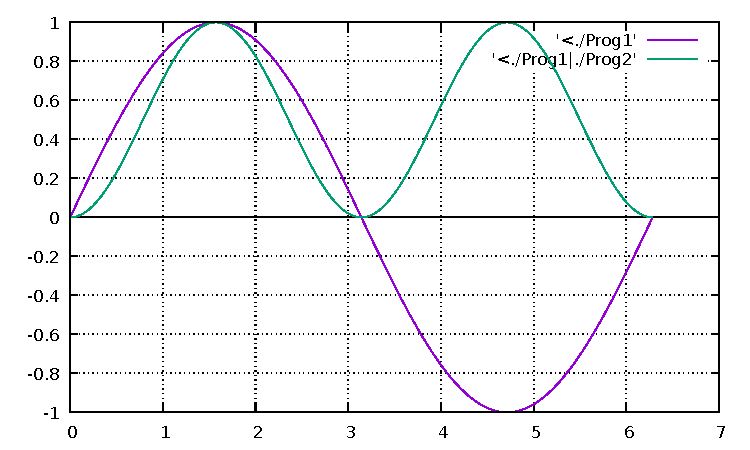
\includegraphics[scale=0.5]{iopipes.pdf}
\end{figure}
\end{frame}

\subsection{Processes and Pipes}
\begin{frame}[fragile]{Processes and Pipes}{Empower your Programming Experience}
  \begin{itemize}
  \item All programs run as processes, interacting with the RAM for
    calculations, and file buffers \& hard drive memory for outputs
    and inputs
  \item Processes are classified as
    \begin{description}
    \item[Parent Process] The process that has called any given
      process
    \item[Child Process] The process that is called by any given
      process
    \end{description}
  \item Use \verb|ps -ef| to see the currently running processes. The
    column PID(2nd column) corresponds to the Process ID of the
    process and the column PPID(3rd column) corresponds to the Parent
    Process ID
  \item All programs are cdhild processes of the \verb|bash|
  \end{itemize}
\end{frame}

\begin{frame}[fragile]{Processes}{An Illustration}
  \begin{center}
    Output of \verb|ps -ef|\\
    Note that the invoked program \verb|ps|, is a child process of
    \verb|bash|\footnote{Short for Bourne again SHell}, which is the
    shell program
  \end{center}
  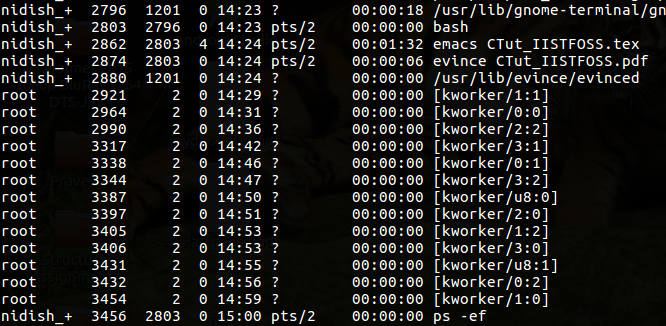
\includegraphics[width=\textwidth]{Processes.png}
\end{frame}

\begin{frame}[fragile]{The fork() function}{Learn to give birth}
  \begin{itemize}
    \item The \verb|fork()| function creates an identical instance of
      the current process
    \item Once the command is issued, the two processes are completely
      distinct
    \item The function has a return value of \verb|pid_t| - fear not!
      This is just an integer type, disguised by typedef
    \item In the parent process the fork function returns the pid of
      the child that is created, and in the child process the function
      returns 0
    \item This may be used to distinguish between the two processes to
      give different instructions to the parent and the child from the
      same source code
  \end{itemize}
\end{frame}

\begin{frame}[fragile]{The fork() function}{An Example}
\begin{verbatim}
#include<stdio.h>
#include<unistd.h>
int main(){
  pid_t fpid,childpid;
  fpid = getpid();
  childpid = fork();
  if( childpid==0 ){
    fprintf(stdout,"I am a child.\n"
	    "My PID is %d.\n"
	    "My Parent's PID is %d.\n\n",getpid(),fpid);}
  else{
    fprintf(stdout,"I am a parent.\n"
	    "My PID is %d.\n"
	    "My Child's PID is %d.\n\n"
            ,getpid(),childpid);}
  return 0;
}   
\end{verbatim}
\end{frame}

\begin{frame}[fragile]{The fork() functions}{An Example}
  \begin{columns}
    \begin{column}{0.5\textwidth}
        \textbf{The Output}
\begin{verbatim}
I am a parent.
My PID is 4672.
My Child's PID is 4673.

I am a child.
My PID is 4673.
My Parent's PID is 4672.

\end{verbatim}
    \end{column}
    \begin{column}{0.5\textwidth}
      \begin{itemize}
        \item Whether the parent or the child is executed first is a
          question we can't address 
        \item The \verb|wait()| function may be use to make the parent
          wait till the child exits and get its exit status - look at
          the corresponding man pages for more
      \end{itemize}
    \end{column}
  \end{columns}
\end{frame}

\begin{frame}[fragile]{The execl() class of functions}{Same name,
    different person}
  \begin{itemize}
    \item The \verb|execl()| class of functions may be used to make
      the current process into an instance of another program (same
      pid, different executable)
    \item The \verb|execl()| function takes as arguments the name of
      the program and the command line arguments (appended by
      \verb|NULL|) that are to be passed to it
      \item An example, to call \verb|ps| with the argument \verb|-ef|
        is,
    \begin{verbatim}
        execl(``ps'',''ps'',''-ef'',NULL);
    \end{verbatim}
    Note that the program name itself is the first argument
  \item Upon failure, the program returns a negative value
  \item This comes in handy when you have different routines that have
    to be implemented on the same set of values which can be passed on
    using command line arguments.
  \end{itemize}
\end{frame}

\begin{frame}[fragile]{Interprocess Communications}{The pipe() Function}
  \begin{itemize}
    \item The pipe() function takes an array of integers as argument
      and writes read and write filedescriptors into them
    \item Say the argument is declared and passed as,
    \begin{verbatim}
      int filedes[2];
      pipe(filedes);
    \end{verbatim}
    \item \verb|filedes[0]| denotes the read file descriptor and
      \verb|filedes[1]| denotes the write file descriptor
      \item Anything written to \verb|filedes[1]| may be read from
        \verb|filedes[0]|
      \item It is sufficient if the file descriptors are somehow
        known to the two processes that are to communicate
      \item In order to make this work with standard output and
        standard input, the \verb|dup2| function may be used to
        duplicate file descriptors
    \end{itemize}
\end{frame}

\begin{frame}[fragile]{Interprocess Communcications}{The dup2()
    Function}
  \begin{itemize}
    \item In order to duplicate the read and write file descriptors as
      \verb|stdin| and \verb|stdout|, the corresponding macros may be
      used,
\begin{verbatim}
  dup2(filedes[0],STDIN_FILENO);
  dup2(filedes[1],STDOUT_FILENO); 
\end{verbatim}
  \item Writing in one process and reading from the other is known as
    half-duplex pipe - it is wise to close the corresponding file
    descriptors in each process using the \verb|close(filedes[k])| call
  \item Writing and reading in/from both processes is known as
    full-duplex pipes - need to be a little careful when dealing with
    these
  \item Examples are given in the attached folder
  \end{itemize}
\end{frame}

\subsection{Working with POSIX Threads}
\begin{frame}[fragile]{POSIX Threads}{Multitask more efficiently}
  \begin{itemize}
    \item Honestly, interprocess communication is a little involved -
      it also involves more overhead
    \item An easier and more efficient way of processing in parallel
      is by using subprocesses, or threads
    \item We introduce the POSIX thread since it is the simplest to
      cover
    \item Each thread has a unique \emph{thread ID} stored in the
      \verb|pthread_t| data type
    \item A thread is created by assigning to it a function and the
      argument that is to be passed
    \item The global variables of the program are shared between all
      the threads and operations may be done on them parallely
    \item There are ways to \emph{lock} the global variable to a
      thread so that none of the others may modify the variable while
      it is operated upon by the current thread
  \end{itemize}
\end{frame}

\begin{frame}[fragile]{POSIX Threads}{Basic Syntax}
  \begin{itemize}
    \item A new thread may be created using the \verb|pthread_create|
      function. It takes as arguments,
      \begin{enumerate}
        \item Address of the variable storing the thread id
        \item pthread options (\verb|NULL| works just fine for
          now) 
        \item \verb|void*| Function to be assigned. This has to have a
          \verb|void*| arg. In C, a \verb|void*| pointer could point
          to virtually ANYTHING
        \item The \verb|void*| argument for the function
      \end{enumerate}
    \item A sample call would be,
\begin{verbatim}
pthread_create(&tid,NULL,function,arg);
\end{verbatim}
    \item The main thread can choose to wait for a particular thread
      to complete execution using the \verb|pthread_join| call which
      takes as arguments the thread id and a pointer to store the
      return variable. If you don't expect to do anything with the
      return variables, just pass \verb|NULL| as below.
\begin{verbatim}
pthread_join(tid,NULL);
\end{verbatim}
  \end{itemize}
\end{frame}

\begin{frame}[fragile]{POSIX Threads}{An Example}
  \begin{columns}
    \begin{column}{0.5\textwidth}
      \textbf{PROGRAM}
\begin{tiny}
\begin{verbatim}
#include<stdio.h>
#include<stdlib.h>
#include<pthread.h>
#include<unistd.h>
void *function(void* a)
{
  int* p = (int*)a;
  fprintf(stdout,"Called Thread"
   " - %d - %d\n",pthread_self(),getpid());  
  return 0;
}
int main()
{
  pthread_t tid;
  int i=10;
  pthread_create(&tid,NULL,function,&i);
  fprintf(stdout,"Primary Thread"
   " - %d - %d\n",pthread_self(),getpid());
  pthread_join(tid,NULL);
  return 0;
}
\end{verbatim}
\end{tiny}
    \end{column}
    \begin{column}{0.5\textwidth}
      {\centering\textbf{OUTPUT}}\\
      \begin{tiny}
\begin{verbatim}
Called Thread - 1697670912 - 2851
Primary Thread - 1705953024 - 2851
\end{verbatim}
      \end{tiny}
      \begin{itemize}
        \item The program creates a thread with the
          \verb|pthread_create| call and after printing it's message,
          waits for the thread to finish with the \verb|pthread_join|
          call
        \item We have also demonstrated the use of the \verb|void*|
          argument under explicit type casting     
      \end{itemize}
    \end{column}
  \end{columns}
\end{frame}

\begin{frame}[fragile]{POSIX Threads}{Mutex Locking I}
  \begin{itemize}
    \item Since the variables are globally defined, there is always
      chance for data corruption
    \item To handle this, we resort to ``locking'' the variables
    \item The mutex class of functions provide one such framework to
      do this
    \item Under this, each thread has to place a lock before it may
      perform an operation. Do note that it is upto the programmer to
      make sure that no thread utilized critical variables without
      locking them - no error would be thrown since this is just a
      framework
    \item A mutex variable may be declared and initialized by,
\begin{verbatim}
pthread_mutex_t lock;
pthread_mutex_init( &lock,NULL );
\end{verbatim}
  \end{itemize}
\end{frame}

\begin{frame}[fragile]{POSIX Threads}{Mutex Locking II}
  \begin{itemize}
    \item The variable \verb|lock| only stores the lock status - it is
      not the shared data
    \item In a thread, a lock may be placed and removed respectively
      by,
\begin{verbatim}
pthread_mutex_lock(&lock);
pthread_mutex_unlock(&lock);
\end{verbatim}
    \item Suppose a sub-thread has placed a lock and the main thread
      has attempted to place one, the main thread waits till the
      sub-thread unlocks
    \item Remember to make sure your thread unlocks before it goes out
      of scope - not doing so may result in a \verb|deadlock| where no
      thread will be able to use the variables
  \end{itemize}
\end{frame}
  
\subsection{Programming With Class}
\begin{frame}[fragile]{Programming With Class}{Swag is for boys, Class is for programmers}
\begin{itemize}
\item When you program, you have to take readability and presentation of the code very seriously - this helps in working on a code for a prolonged time
\item There are some tools which help us do this effectively
\item For starters, \verb|GNU make| helps us streamline the compilation and linking process
\item Although \verb|make| is beyond the scope of the current presentation, a few tips may be noted:
\item Organize your project directory into subdirectories \verb|src/|, \verb|obj/|, \verb|include/|, \verb|bin/|, and \verb|examples/|.
\item Store your ".c" files in \verb|src/|, ".o" files in \verb|obj/|, ".h" (and corresponding ".c") files in \verb|include/|, executables in \verb|bin/| and \verb|examples/|
\item The \verb|example/| folder may be used for test runs - A \verb|Makefile| in the root will make all this very handy
\end{itemize}
\end{frame}

\begin{frame}[fragile]{Programming With Class}{Building your first library}
\begin{columns}
\begin{column}{0.5\textwidth}
\textbf{library.h}
\begin{verbatim}
#ifndef LIB_DEFD
#define LIB_DEFD

double square(double);
double cube(double);

#endif
\end{verbatim}
\end{column}
\begin{column}{0.5\textwidth}
\textbf{library.c}
\begin{verbatim}
#include<library.h>
double square(double a)
{  return a*a; }

double cube(double a)
{  return a*a*a; }
\end{verbatim}
\end{column}
\end{columns}
\begin{itemize}
\item Consider the above ".h" file with two functions \verb|square()| and \verb|cube()|
\item They are declared in \verb|library.h| and defined in \verb|library.c|
\end{itemize}
\end{frame}

\begin{frame}[fragile]{Programming With Class}{Building your first library}
\begin{itemize}
\item In order to make this a library, we first make an object file by running, \verb|$ gcc -c library.c -I.| [\verb|-I.| denotes that \verb|library.h| is in the current directory]
\item This creates \verb|library.o|, the corresponding object file
\item We add this to an archive file, \verb|libtest.a| by, \verb|$ ar cr libtest.a library.o|
\item Any number of object files may be added to an archive file. So you may have one small header file with only declarations and numerous \verb|.c| files where one may find the function definitions
\item Linking this to a program is easy, chuck the \verb|lib| and the \verb|.a| parts and give the rest of the name with a \verb|-l| flag preceded by \verb|-L.| specifying where the archive is,
\begin{verbatim}
$ gcc Main.c -L. -ltest -I. -o Run
\end{verbatim}
\end{itemize}
\begin{small}
Sample programs may be found in a directory attached herewith
\end{small}
\end{frame}

\subsection*{References}
\begin{frame}[fragile]{References}
\begin{thebibliography}{2}
\bibitem{man} Linux \verb|man| pages
\end{thebibliography}
\end{frame}

\section{Some Useful Libraries}
\begin{frame}{Some Useful Libraries}{Something worth your time}
\begin{description}
\item[FFTW] (Fastest Fourier Transform in the West) No idea about the name - but comes in really handly for signal processing and other applications
\item[GSL] (GNU Scientific Library) Another GNU produce - indispensable for my everyday existence - has got just about anything you might need
\item[GL,GLU,GLUT] (OpenGL class of Libraries) A very handy library to be abreast of the basics of - opened my eyes, I should say
\end{description}
\end{frame}

\end{document}
